%!TeX program = pdflatex
% Geoff Boeing's Curriculum Vitae
% Email: boeing@usc.edu
% Web: https://geoffboeing.com/
% Repo: https://github.com/gboeing/cv

\documentclass[12pt,letterpaper]{report}

%\usepackage{simplecv}

\usepackage[T1]{fontenc} % output T1 font encoding (8-bit) for accented characters as single glyph
\usepackage[strict,autostyle]{csquotes} % smart and nestable quote marks
\usepackage[USenglish]{babel} % regionalize hyphens, quote marks, etc automatically
\usepackage{microtype}% improve text appearance with kerning, etc
\usepackage{datetime} % enable formatting of date output
\usepackage{tabto}    % make nice tabbing
\usepackage{hyperref} % enable hyperlinks and pdf metadata
\usepackage{geometry} % manually set page margins
\usepackage{enumitem} % enumerate with [resume] option
\usepackage{titlesec} % allow custom section fonts
\usepackage{setspace} % custom line spacing

\usepackage{graphicx}
\newcommand{\headingphoto}[3]{
	\begin{minipage}[t]{0.60\textwidth}
		\begin{dummyenv}
			\vspace*{\fill}
			\Huge \textcolor{color-title}{#1}
		\end{dummyenv}
		\vspace{5mm}\\
		#2
	\end{minipage}
	\begin{minipage}[t]{0.35\textwidth}
		\begin{flushright}
			\includegraphics[width=1.67\linewidth,keepaspectratio,valign=t]{#3}
		\end{flushright}
	\end{minipage}
}

% what is your name?
\newcommand{\myname}{Zhaohui Huang}

% select default typefaces
\usepackage{ebgaramond} % document's serif typeface
\usepackage{tgheros}    % document's sans serif typeface

% how far to tab for list items with left-aligned date: different fonts need different widths
\newcommand{\listtabwidth}{1.7cm}

% define font to use as document's title
\newcommand{\namefont}[1]{{\normalfont\bfseries\Huge{#1}}}

% set section heading fonts and before/after spacing
\SetTracking{encoding=*, family=\sfdefault}{30} % increase sans serif headings tracking
\titleformat{\section}{\lsstyle\sffamily\small\bfseries\uppercase}{}{}{}{}
\titlespacing{\section}{0pt}{30pt plus 4pt minus 4pt}{8pt plus 2pt minus 2pt}

% set subsection heading fonts and before/after spacing
\titleformat{\subsection}{\lsstyle\sffamily\footnotesize\bfseries}{}{}{}{}
\titlespacing{\subsection}{0pt}{16pt plus 4pt minus 4pt}{4pt plus 2pt minus 2pt}

% set page margins (assumes letter paper)
\geometry{body={6.5in, 9.0in},
    left=1.0in,
    top=1.0in}

% prevent paragraph indentation
\setlength\parindent{0em}

% set line spacing
\setstretch{0.9}

% define space between list items
\newcommand{\listitemspace}{0.25em}

% make unordered lists without bullets and use compact spacing
\renewenvironment{itemize}
{\begin{list}{}{\setlength{\leftmargin}{0em}
                \setlength{\parskip}{0em}
                \setlength{\itemsep}{\listitemspace}
                \setlength{\parsep}{\listitemspace}}}
{\end{list}}

% make tabbed lists so content is left-aligned next to years
\TabPositions{\listtabwidth}
\newlist{tablist}{description}{3}
\setlist[tablist]{leftmargin=\listtabwidth,
    labelindent=0em,
    topsep=0em,
    partopsep=0em,
    itemsep=\listitemspace,
    parsep=\listitemspace,
    font=\normalfont}

% print only the month and year when using \today
\newdateformat{monthyeardate}{\monthname[\THEMONTH] \THEYEAR}

% define hyperlink appearance and metadata for pdf properties
\hypersetup{
    colorlinks  = true,
    urlcolor    = black,
    citecolor   = black,
    linkcolor   = black,
    pdfauthor   = {\myname},
    pdfkeywords = {city planning, housing, street networks, transportation, urban design, urban informatics},
    pdftitle    = {\myname: Curriculum Vitae},
    pdfsubject  = {Curriculum Vitae},
    pdfpagemode = UseNone
}

\begin{document}
    \raggedright{}

    % display your name as the document title
    \namefont{\myname}
    

    % affiliation and contact info blocks
    \vspace{1em}
    \begin{minipage}[t]{0.700\textwidth}
        % current primary affiliation, left-aligned
        \
        \newline
        \
        \newline
        

        Department of Mechanics and Engineering Science \\
        College of Enigneering, Peking University \\
        Beijing, 100871, China
        \
        \newline
        
        Email: \href{mailto:2001111696@pku.edu.cn}{2001111696@pku.edu.cn} \\
        Phone: +86 18811711781
        
    \end{minipage}
	%\centering{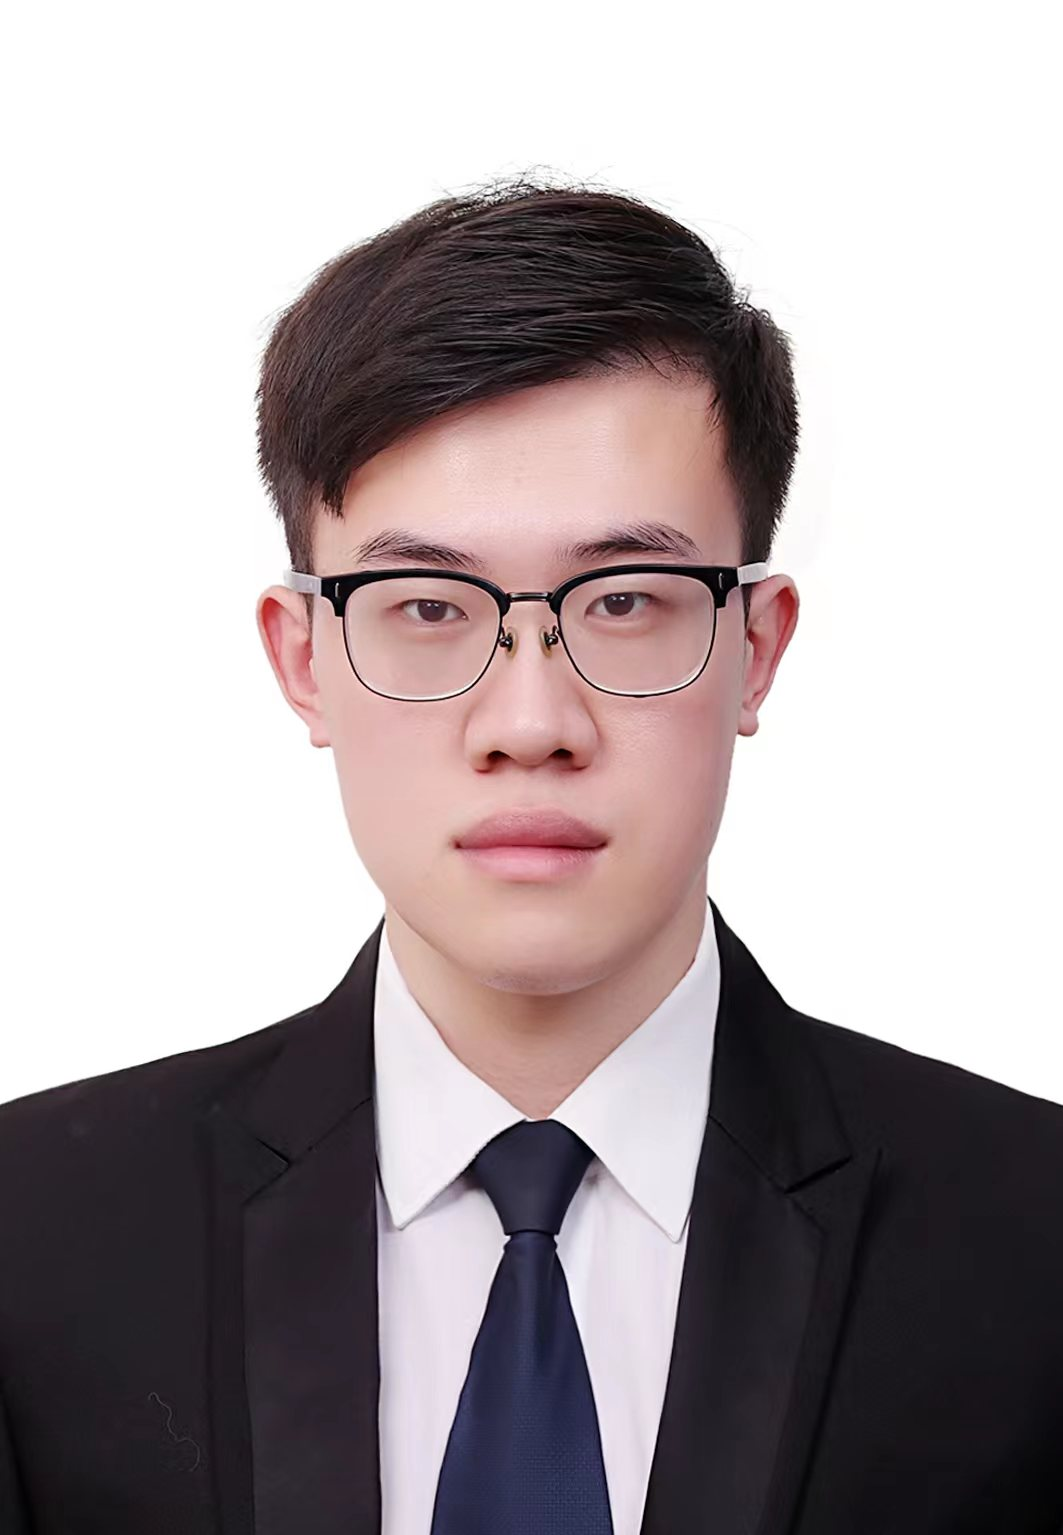
\includegraphics[scale=0.3]{photo1.jpg}}
    \begin{minipage}[t]{0.295\textwidth}
        % contact info details, right-aligned
        \headingphoto{}{
        }{photo1.jpg}
    	%\centering{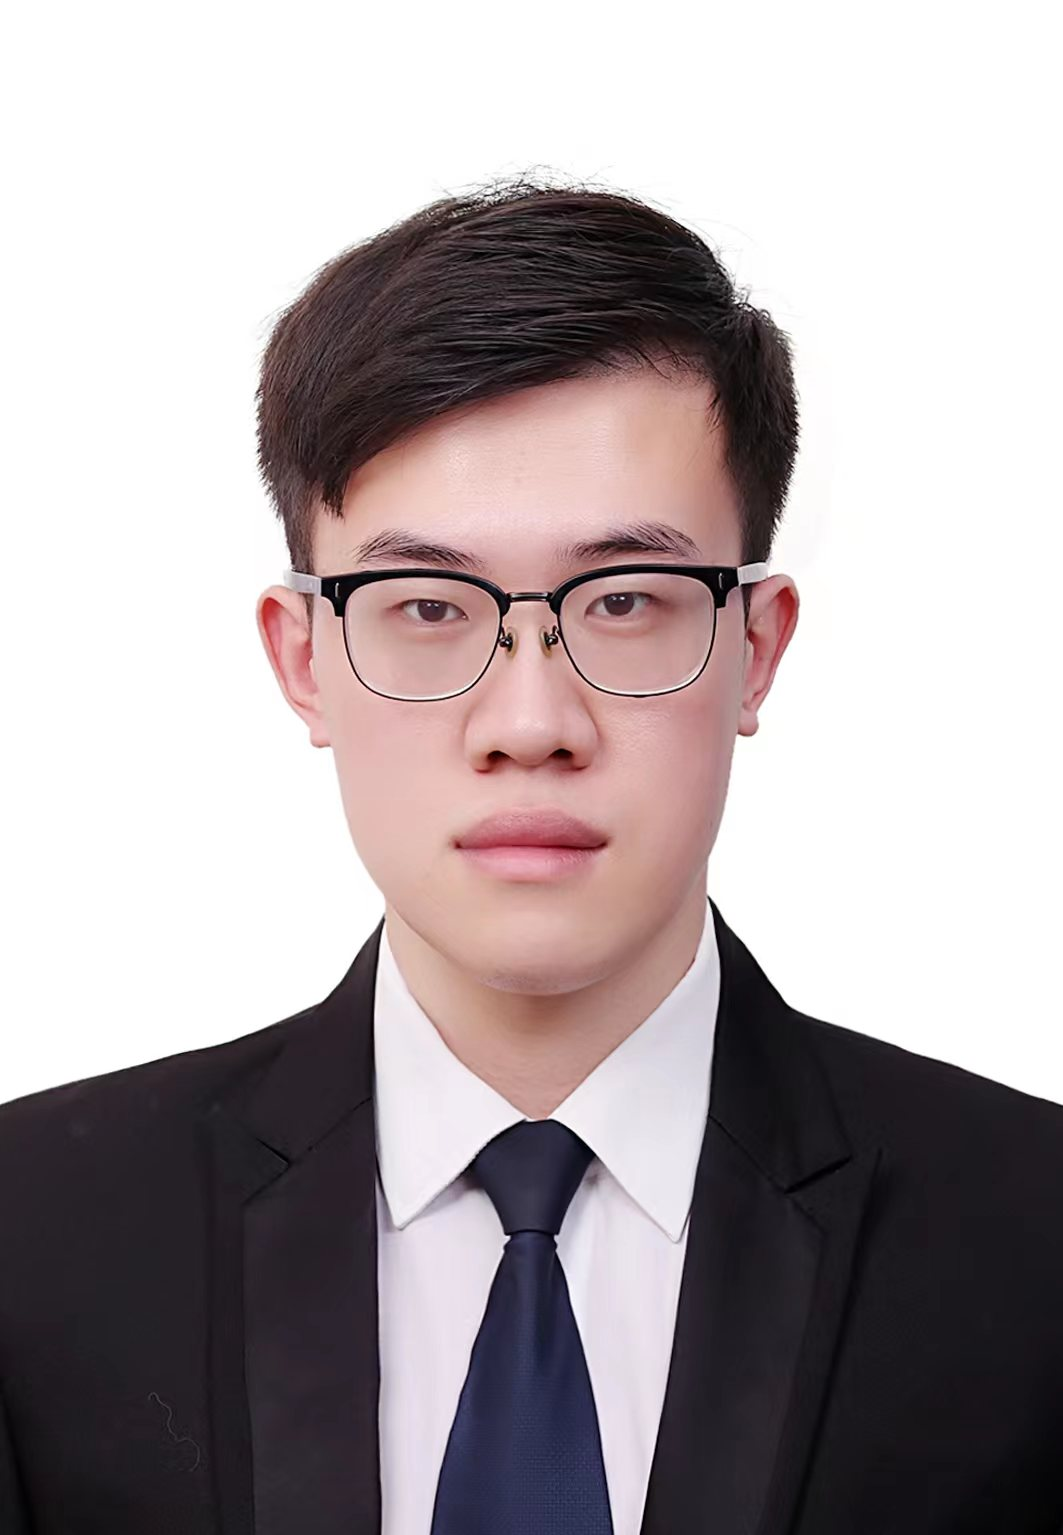
\includegraphics[width=.5\linewidth,keepaspectratio,valign=t]{photo1.jpg}}
        \flushright{}
    \end{minipage}


    \section*{Education}

    \begin{tablist}

        \item[Ph.D.] \tab{}Engineering Mechanics, Peking University, 2020-present
        \item[B.S.]  \tab{}Theoretical and Applied Mechanics, Peking University, 2016-2020

    \end{tablist}

	\section*{PROFESSIONAL EXPERIENCE}

	\subsection*{Teaching Assistant}

	\begin{tablist}

		\item[2021] \tab{}Computational Methods (Undergrad. Level), Peking Univeristy

		\item[2020] \tab{}Engineering CAD (Undergrad. Level), Peking University

	\end{tablist}

    \section*{Research Areas}

    \begin{itemize}

        \item 1. Granular materials: jammed packings of non-spherical particles and mechanical properties.
        \item 2. Inverse design of materials: the pursuit of perfect packings and geometrically densest packings.

    \end{itemize}



    



	\section*{Publications}
	
	\subsection*{Journal Articles}
	
	\begin{tablist}
		
		\item[2023] \tab{}\textbf{Huang Z}, Deng W, Zhang S, et al. \enquote{Optimal shapes of disk assembly in saturated random packings.} \textit{Physical Chemistry Chemical Physics}, \textbf{forthcoming}.
		
		\item[2022] \tab{}Wang Y, Deng W, \textbf {Huang Z}, et al. \enquote{Descriptor-free unsupervised learning method for local structure identification in particle packings.} \textit{The Journal of Chemical Physics}, 2022, 156(15): 154504. \href{https://doi.org/10.1063/5.0088056}{https://doi.org/10.1063/5.0088056}
		
		\item[2021] \tab{}\textbf{Huang Z}, Deng W, Yuan Y, et al. \enquote{Determining the equivalent packing diameter of two-dimensional shapes.} \textit{Powder Technology}, 2022, 396: 565-577. \href{https://doi.org/10.1016/j.powtec.2021.11.022}{https://doi.org/10.1016/j.powtec.2021.11.022}
		
		
	\end{tablist}
	
	\subsection*{Working Papers}
	
	\begin{tablist}
		
		\textbf{Huang Z}, Zhou X, Jin W, et al. \enquote{Shape and space filling: a review on particle packing.}
		
		
	\end{tablist}
	
	\section*{Conference Activity}
	
	\begin{tablist}
		
		\item[2022] \tab{}12th Natl. Conf. on Soft Matter and Biological Physics. Wenzhou, China.
		
		\item[2021] \tab{}Chinese Physical Society Fall Metting. Lanzhou, China.
		
	\end{tablist}
	
	
	
	
	
	\section*{SCIENTIFIC COMPUTING}
	
	\subsection*{ Programming}
	
	\begin{tablist}
		
		C++, C, Python, TeX.
	\end{tablist}
	
	\subsection*{Software}
	
	\begin{tablist}
		
		 experience in Auto CAD, Ovito, etc.
		
	\end{tablist}

	\section*{Awards}
	
	\begin{tablist}
		
		\item[2022] \tab{}Lee Wai Wing Scholarship
		
		\item[2021] \tab{}Outstanding Research Award
		
	\end{tablist}
	
	
	
	
	\end{document}
